\documentclass[10pt,aspectratio=169,serif,fleqn]{beamer}

\usepackage[fontset=none, scheme=plain]{ctex}
\IfFontExistsTF{Songti SC}{%
	\setCJKmainfont{Songti SC}[AutoFakeSlant=0.2]%
	\setCJKsansfont{Songti SC}[AutoFakeSlant=0.2]%
}{%
	\setCJKmainfont{FandolSong-Regular}[Extension=.otf,BoldFont=FandolSong-Bold,AutoFakeSlant=0.2]%
	\setCJKsansfont{FandolSong-Regular}[Extension=.otf,BoldFont=FandolSong-Bold]%
}
\usepackage{amsmath,amssymb,graphicx,tikz,booktabs,multicol,calligra}
\usepackage{pgfplots}
\pgfplotsset{compat=1.18}
\usepackage{tcolorbox}
\tcbuselibrary{skins}
\usepackage{XyygU}
\usepackage{caption}
\captionsetup[figure]{name=图,labelsep=period}

\usetikzlibrary{arrows.meta,positioning,calc}

\setlength{\abovedisplayskip}{0pt plus 2pt minus 2pt}
\setlength{\belowdisplayskip}{0pt plus 2pt minus 2pt}

\title[习题3.2]{习题3.2 \quad 单调性与最大（小）值、奇偶性}
\subtitle{复习巩固 \& 综合运用 \& 拓广探索}
\author{}
\institute{}
\date{2026-10-23}

\begin{document}

\begin{frame}
  \titlepage
\end{frame}

% ========== 第1题 ==========
\section{复习巩固}
\begin{frame}[t]{第1题：由图象说单调区间}
\textbf{1.} 根据下图说出函数的单调区间及在每一单调区间上的单调性。

\vspace{0.5em}
\begin{center}
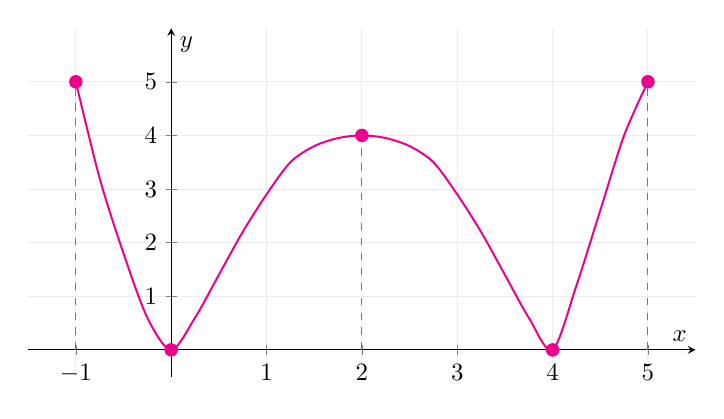
\begin{tikzpicture}[scale=0.9]
\begin{axis}[
    width=11cm, height=6.5cm,
    axis lines=middle,
    xlabel=$x$, ylabel=$y$,
    xmin=-1.5, xmax=5.5, ymin=-0.5, ymax=6,
    xtick={-1,0,1,2,3,4,5},
    ytick={1,2,3,4,5},
    grid=major, grid style={gray!15},
]
% 精确测定的坐标点（0到4区间加密，峰顶在x=2）
\addplot[thick,magenta,smooth] coordinates {
    (-1,5)
    (-0.75,3.2)
    (-0.5,1.8)
    (-0.25,0.6)
    (0,0)
    (0.25,0.6)
    (0.5,1.4)
    (0.75,2.2)
    (1,2.9)
    (1.25,3.5)
    (1.5,3.8)
    (1.75,3.95)
    (2,4)
    (2.25,3.95)
    (2.5,3.8)
    (2.75,3.5)
    (3,2.9)
    (3.25,2.2)
    (3.5,1.4)
    (3.75,0.6)
    (4,0)
    (4.25,1.2)
    (4.5,2.6)
    (4.75,4.0)
    (5,5)
};
% 端点标记
\addplot[only marks,mark=*,mark size=2.5pt,magenta] coordinates {(-1,5)(0,0)(2,4)(4,0)(5,5)};
% 垂直虚线到x轴
\draw[dashed,blue!60] (axis cs:-1,0) -- (axis cs:-1,5);
\draw[dashed,blue!60] (axis cs:2,0) -- (axis cs:2,4);
\draw[dashed,blue!60] (axis cs:4,0) -- (axis cs:4,0);
\draw[dashed,blue!60] (axis cs:5,0) -- (axis cs:5,5);
\end{axis}
\end{tikzpicture}
\end{center}
\end{frame}

\begin{frame}[t]{第1题 解答}
\begin{tcolorbox}[colback=orange!10,colframe=orange,title=\textbf{解}]
函数的单调区间有：$[-1,0]$，$[0,2]$，$[2,4]$，$[4,5]$。

\vspace{0.5em}
\begin{itemize}
  \item 在区间 $[-1,0]$ 上，图象下降，函数 \alert{单调递减}；
  \item 在区间 $[0,2]$ 上，图象上升，函数 \alert{单调递增}；
  \item 在区间 $[2,4]$ 上，图象下降，函数 \alert{单调递减}；
  \item 在区间 $[4,5]$ 上，图象上升，函数 \alert{单调递增}。
\end{itemize}
\end{tcolorbox}
\end{frame}

% ========== 第2题 ==========
\begin{frame}[t]{第2题：画图象说单调区间}
\textbf{2.} 画出下列函数的图象，并根据图象说出函数 $y=f(x)$ 的单调区间及在每一单调区间上的单调性。

\vspace{0.5em}
(1) $y=x^2-5x-6$；\hfil (2) $y=9-x^2$。
\end{frame}

\begin{frame}[t]{第2题 解答}
\begin{tcolorbox}[colback=orange!10,colframe=orange,title=\textbf{解}]
(1) $y=x^2-5x-6=\left(x-\dfrac52\right)^2-\dfrac{49}{4}$，开口向上，对称轴 $x=\dfrac52$。

\vspace{0.3em}
单调递减区间：$\left(-\infty,\dfrac52\right]$；单调递增区间：$\left[\dfrac52,+\infty\right)$。

\vspace{0.8em}
(2) $y=9-x^2$，开口向下，对称轴 $x=0$。

\vspace{0.3em}
单调递增区间：$(-\infty,0]$；单调递减区间：$[0,+\infty)$。
\end{tcolorbox}
\end{frame}

\begin{frame}[t]{第2题 图象}
\begin{center}
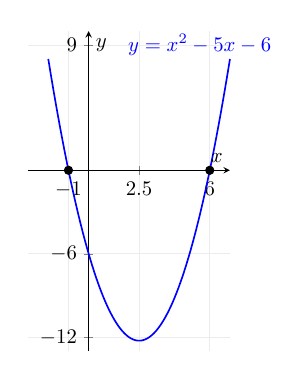
\begin{tikzpicture}[scale=0.75]
\begin{axis}[
	clip=false,
    width=5cm, height=7cm,
    axis lines=middle,
    xlabel=$x$, ylabel=$y$,
    xmin=-3, xmax=7, ymin=-13, ymax=10,
    xtick={-1,2.5,6},
    ytick={-12,-6,9},
    grid=major, grid style={gray!15},
]
\addplot[thick,blue,domain=-2:7,samples=80] {x^2-5*x-6};
\addplot[mark=*,mark size=2pt,mark color=blue] coordinates {(-1,0) (6,0)};
\node[blue] at (axis cs:5.5,9) {$y=x^2-5x-6$};

\end{axis}
\end{tikzpicture}
\hspace{2cm}
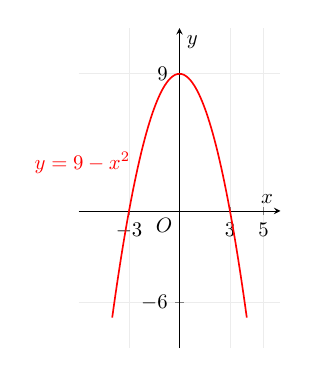
\begin{tikzpicture}[scale=0.75]
	\begin{axis}[
		clip=false,
		width=5cm, height=7cm,
		axis lines=middle,
		xlabel=$x$, ylabel=$y$,
		xmin=-6, xmax=6, ymin=-9, ymax=12,
		xtick={-3,3,5},
		ytick={-12,-6,9},
		grid=major, grid style={gray!15},
		]
		
		\addplot[thick,red,domain=-4:4,samples=80] {9-x^2};
		\node[below left] at (axis cs:0,0) {$O$};
		

		\node[red,above left] at (axis cs:-2.5,2) {$y=9-x^2$};
	\end{axis}
\end{tikzpicture}
\end{center}
\end{frame}

% ========== 第3题 ==========
\begin{frame}[t]{第3题：用定义证明单调性}
\textbf{3.} 证明：

(1) 函数 $f(x)=-2x+1$ 是减函数；

(2) 函数 $f(x)=x^2+1$ 在 $(0,+\infty)$ 上单调递增；

(3) 函数 $f(x)=1-\dfrac{1}{x}$ 在 $(-\infty,0)$ 上单调递增。
\end{frame}

\begin{frame}[t]{第3题 解答}
\begin{tcolorbox}[colback=orange!10,colframe=orange,title=\textbf{解}]
(1) 任取 $x_1<x_2\in\mathbf{R}$，
\[
f(x_1)-f(x_2)=(-2x_1+1)-(-2x_2+1)=2(x_2-x_1)>0,
\]
即 $f(x_1)>f(x_2)$，故 $f(x)=-2x+1$ 是减函数。

\vspace{0.5em}
(2) 任取 $0<x_1<x_2$，
\[
f(x_1)-f(x_2)=x_1^2-x_2^2=(x_1-x_2)(x_1+x_2)<0,
\]
即 $f(x_1)<f(x_2)$，故在 $(0,+\infty)$ 上单调递增。
\end{tcolorbox}
\end{frame}

\begin{frame}[t]{第3题 解答：(3)}
\begin{tcolorbox}[colback=orange!10,colframe=orange,title=\textbf{解：(3)}]
任取 $x_1<x_2<0$，
\[
f(x_1)-f(x_2)=\left(1-\frac1{x_1}\right)-\left(1-\frac1{x_2}\right)=\frac1{x_2}-\frac1{x_1}=\frac{x_1-x_2}{x_1x_2}.
\]
因为 $x_1<x_2<0$，所以 $x_1-x_2<0$，$x_1x_2>0$，
\[
f(x_1)-f(x_2)=\frac{x_1-x_2}{x_1x_2}<0,
\]
即 $f(x_1)<f(x_2)$，故 $f(x)=1-\dfrac1x$ 在 $(-\infty,0)$ 上单调递增。
\end{tcolorbox}
\end{frame}

% ========== 第4题 ==========
\begin{frame}[t]{第4题：汽车租赁月收益}
\textbf{4.} 某汽车租赁公司的月收益 $y$（单位：元）与每辆车的月租金 $x$（单位：元）间的关系为
\[
y=-\frac{x^2}{50}+162x-21000,
\]
那么，每辆车的月租金为多少元时，租赁公司的月收益最大？最大月收益是多少？
\end{frame}

\begin{frame}[t]{第4题 解答}
\begin{tcolorbox}[colback=orange!10,colframe=orange,title=\textbf{解}]
$y=-\dfrac1{50}(x^2-8100x)-21000$，
\[
y=-\frac1{50}(x-4050)^2+\frac{4050^2}{50}-21000.
\]
当 $x=4050$ 时，$y$ 取最大值：
\[
y_{\max}=\frac{16402500}{50}-21000=328050-21000=307050.
\]
\vspace{0.3em}
所以当月租金定为 \alert{4050 元}时，月收益最大，最大月收益为 \alert{307050 元}。
\end{tcolorbox}
\end{frame}

% ========== 第5题 ==========
\begin{frame}[t]{第5题：判断奇偶性}
\textbf{5.} 判断下列函数的奇偶性：

\vspace{0.5em}
(1) $f(x)=x^2+1$；\hfil (2) $f(x)=\dfrac{x}{x^2+1}$。
\end{frame}

\begin{frame}[t]{第5题 解答}
\begin{tcolorbox}[colback=orange!10,colframe=orange,title=\textbf{解}]
(1) 定义域为 $\mathbf{R}$，关于原点对称。
\[
f(-x)=(-x)^2+1=x^2+1=f(x),
\]
故 $f(x)=x^2+1$ 是 \alert{偶函数}。

\vspace{0.8em}
(2) 定义域为 $\mathbf{R}$，关于原点对称。
\[
f(-x)=\frac{-x}{(-x)^2+1}=-\frac{x}{x^2+1}=-f(x),
\]
故 $f(x)=\dfrac{x}{x^2+1}$ 是 \alert{奇函数}。
\end{tcolorbox}
\end{frame}

% ========== 第6题 ==========
\section{综合应用}
\begin{frame}[t]{第6题：心率随时间变化}
\textbf{6.} 一名心率过速患者服用某种药物后心率立刻明显减慢，之后随着药力的减退，心率再次慢慢升高。画出自服药那一刻起，心率关于时间的一个可能的图象（示意图）。
\end{frame}

\begin{frame}[t]{第6题 参考图象}
\begin{center}
\begin{tikzpicture}[scale=0.9]
\begin{axis}[
    width=12cm, height=6cm,
    axis lines=middle,
    xlabel=$t$, ylabel=$心率$,
    xmin=0, xmax=10, ymin=50, ymax=120,
    xtick=\empty,
    ytick={60,80,100,120},
    grid=major, grid style={gray!15},
]
\addplot[thick,blue,domain=0:10,samples=100] {100-40*exp(-(x-1)^2*0.6)+1.5*x};
\node[blue,above right] at (axis cs:0.2,100) {服药};
\end{axis}
\end{tikzpicture}
\end{center}
\end{frame}

% ========== 第7题 ==========
\begin{frame}[t]{第7题：二次函数的单调区间与最值}
\textbf{7.} 已知函数 $f(x)=x^2-2x$，$g(x)=x^2-2x\ (x\in[2,4])$，

(1) 求 $f(x)$，$g(x)$ 的单调区间；

(2) 求 $f(x)$，$g(x)$ 的最小值。
\end{frame}

\begin{frame}[t]{第7题 解答}
\begin{tcolorbox}[colback=orange!10,colframe=orange,title=\textbf{解}]
$f(x)=x^2-2x=(x-1)^2-1$，对称轴 $x=1$。

\vspace{0.3em}
(1) $f(x)$ 单调递减区间 $(-\infty,1]$，单调递增区间 $[1,+\infty)$；

\vspace{0.3em}
$g(x)$ 定义域 $[2,4]$ 在对称轴右侧，故 $g(x)$ 在 $[2,4]$ 上 \alert{单调递增}。

\vspace{0.8em}
(2) $f(x)$ 在 $x=1$ 处取最小值 $f(1)=-1$；

$g(x)$ 在 $x=2$ 处取最小值 $g(2)=4-4=0$。
\end{tcolorbox}
\end{frame}

% ========== 第8题 ==========
\begin{frame}[t]{第8题：对勾函数的单调性}
\textbf{8.} (1) 根据函数单调性的定义证明函数 $y=x+\dfrac{9}{x}$ 在区间 $[3,+\infty)$ 上单调递增。

\vspace{0.5em}
(2) 讨论函数 $y=x+\dfrac{9}{x}$ 在区间 $(0,+\infty)$ 上的单调性。

\vspace{0.5em}
(3) 讨论函数 $y=x+\dfrac{k}{x}\ (k>0)$ 在区间 $(0,+\infty)$ 上的单调性。
\end{frame}

\begin{frame}[t]{第8题 解答：(1)(2)}\vspace{-2em}
\begin{tcolorbox}[colback=orange!10,colframe=orange,title=\textbf{解}]
(1) 任取 $3\le x_1<x_2$，
\[
f(x_1)-f(x_2)=(x_1-x_2)+9\left(\frac1{x_1}-\frac1{x_2}\right)=(x_1-x_2)\left(1-\frac{9}{x_1x_2}\right).
\]
因 $x_1<x_2$，$x_1-x_2<0$；又 $x_1,x_2\ge3$，故 $x_1x_2\ge9$，$1-\dfrac{9}{x_1x_2}\ge0$。

\vspace{0.3em}
所以 $f(x_1)-f(x_2)\le0$，即 $f(x_1)\le f(x_2)$，$f(x)$ 在 $[3,+\infty)$ 上单调递增。

\vspace{0.8em}
(2) 同理，当 $0<x_1<x_2\le3$ 时 $x_1x_2<9$，$1-\dfrac{9}{x_1x_2}<0$，$f(x_1)-f(x_2)>0$，递减。

\vspace{0.3em}
故 $y=x+\dfrac9x$ 在 $(0,3]$ 上单调递减，在 $[3,+\infty)$ 上单调递增。
\end{tcolorbox}
\end{frame}

\begin{frame}[t]{第8题 解答：(3)}
\begin{tcolorbox}[colback=orange!10,colframe=orange,title=\textbf{解：(3)}]
对 $y=x+\dfrac{k}{x}\ (k>0)$，任取 $0<x_1<x_2$：
\[
f(x_1)-f(x_2)=(x_1-x_2)\left(1-\frac{k}{x_1x_2}\right).
\]

\vspace{0.5em}
当 $x_1x_2>k$，即 $x_1,x_2>\sqrt{k}$ 时，$1-\dfrac{k}{x_1x_2}>0$，$f(x_1)<f(x_2)$，递增；

\vspace{0.5em}
当 $x_1x_2<k$，即 $0<x_1<x_2<\sqrt{k}$ 时，$f(x_1)>f(x_2)$，递减。

\vspace{0.5em}
\textbf{结论：} $y=x+\dfrac{k}{x}$ 在 $(0,\sqrt{k}]$ 上单调递减，在 $[\sqrt{k},+\infty)$ 上单调递增。
\end{tcolorbox}
\end{frame}

% ========== 第9题 ==========
\begin{frame}[t]{第9题：单调性的等价刻画}
\textbf{9.} 设函数 $y=f(x)$ 的定义域为 $D$，区间 $I\subseteq D$，记 $\Delta x=x_1-x_2$，$\Delta y=f(x_1)-f(x_2)$。证明：

(1) 函数 $y=f(x)$ 在区间 $I$ 上单调递增的充要条件是：$\forall x_1,x_2\in I$，$x_1\ne x_2$，都有 $\dfrac{\Delta y}{\Delta x}>0$；

(2) 函数 $y=f(x)$ 在区间 $I$ 上单调递减的充要条件是：$\forall x_1,x_2\in I$，$x_1\ne x_2$，都有 $\dfrac{\Delta y}{\Delta x}<0$。
\end{frame}

\begin{frame}[t]{第9题 解答}
\begin{tcolorbox}[colback=orange!10,colframe=orange,title=\textbf{证明}]
(1) \textbf{必要性：} 若 $f$ 在 $I$ 上递增，则 $x_1<x_2\Rightarrow f(x_1)<f(x_2)$。

\vspace{0.3em}
$\Delta x=x_1-x_2<0$，$\Delta y=f(x_1)-f(x_2)<0$，故 $\dfrac{\Delta y}{\Delta x}>0$。

\vspace{0.5em}
\textbf{充分性：} 若 $\dfrac{\Delta y}{\Delta x}>0$，则 $\Delta y$ 与 $\Delta x$ 同号。

\vspace{0.3em}
当 $x_1<x_2$，即 $\Delta x<0$ 时，$\Delta y<0$，即 $f(x_1)<f(x_2)$，故 $f$ 在 $I$ 上递增。

\vspace{0.8em}
(2) 同理，递减时 $\Delta x$ 与 $\Delta y$ 异号，$\dfrac{\Delta y}{\Delta x}<0$，反之亦然。
\end{tcolorbox}
\end{frame}

% ========== 第10题 ==========
\begin{frame}[t]{第10题：熊猫居室面积}
\textbf{10.} 如图所示，动物园要建造一面靠墙的两间面积相同的矩形熊猫居室，如果可供建造围墙的材料总长是 $30$ m，那么宽 $x$（单位：m）为多少时才能使所建造的每间熊猫居室面积最大？每间熊猫居室的最大面积是多少？
\end{frame}

\begin{frame}[t]{第10题 解答}
\begin{tcolorbox}[colback=orange!10,colframe=orange,title=\textbf{解}]
如图，两间居室并排，共需 $3$ 段宽 $x$ 和 $1$ 段总长（平行于墙）。

\vspace{0.3em}
设平行于墙的总长为 $y$，则 $3x+y=30$，即 $y=30-3x$。

\vspace{0.3em}
两间总面积 $S=xy=x(30-3x)=-3x^2+30x=-3(x-5)^2+75$。

\vspace{0.5em}
当 $x=5$ 时，总面积最大为 $75\,\text{m}^2$，每间最大面积为 $\dfrac{75}{2}=37.5\,\text{m}^2$。

\vspace{0.5em}
故宽 $x=\alert{5\,\text{m}}$ 时每间居室面积最大，最大面积为 $\alert{37.5\,\text{m}^2}$。
\end{tcolorbox}
\end{frame}

% ========== 第11题 ==========
\begin{frame}[t]{第11题：由奇函数求解析式}
\textbf{11.} 已知函数 $f(x)$ 是定义域为 $\mathbf{R}$ 的奇函数，当 $x\ge 0$ 时，$f(x)=x(1+x)$。画出函数 $f(x)$ 的图象，并求出函数的解析式。
\end{frame}

\begin{frame}[t]{第11题 解答}
\begin{tcolorbox}[colback=orange!10,colframe=orange,title=\textbf{解}]
当 $x<0$ 时，$-x>0$，由奇函数：
\[
f(x)=-f(-x)=-[(-x)(1+(-x))]=x(1-x).
\]
又 $f(0)=0$，故
\[
f(x)=
\begin{cases}
x(1+x), & x\ge 0,\\
x(1-x), & x<0.
\end{cases}
\]
\end{tcolorbox}
\end{frame}

\begin{frame}[t]{第11题 图象}
\begin{center}
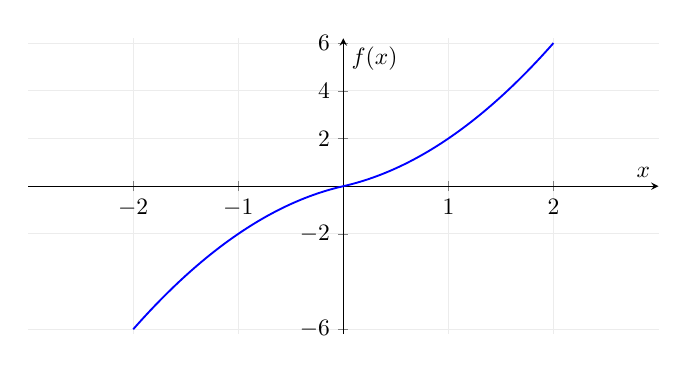
\begin{tikzpicture}[scale=0.85]
\begin{axis}[
    width=11cm, height=6cm,
    axis lines=middle,
    xlabel=$x$, ylabel=$f(x)$,
    xmin=-3, xmax=3, ymin=-6.2, ymax=6.2,
    xtick={-2,-1,0,1,2},
    ytick={-6,-2,0,2,4,6},
    grid=major, grid style={gray!15},
]
\addplot[thick,blue,domain=0:2,samples=50] {x*(1+x)};
\addplot[thick,blue,domain=-2:0,samples=50] {x*(1-x)};
\end{axis}
\end{tikzpicture}
\end{center}
\end{frame}

% ========== 第12题 ==========
\section{拓广探索}
\begin{frame}[t]{第12题：偶函数的单调区间对称}
\textbf{12.} 已知函数 $f(x)$ 是偶函数，而且在 $(0,+\infty)$ 上单调递减，判断 $f(x)$ 在 $(-\infty,0)$ 上单调递增还是单调递减，并证明你的判断。
\end{frame}

\begin{frame}[t]{第12题 解答}
\begin{tcolorbox}[colback=orange!10,colframe=orange,title=\textbf{解}]
$f(x)$ 在 $(-\infty,0)$ 上 \alert{单调递增}。

\vspace{0.5em}
\textbf{证明：} 任取 $x_1<x_2<0$，则 $-x_1>-x_2>0$。

\vspace{0.3em}
因为 $f(x)$ 在 $(0,+\infty)$ 上递减，所以
\[
f(-x_1)<f(-x_2).
\]
又 $f(x)$ 为偶函数，$f(-x_1)=f(x_1)$，$f(-x_2)=f(x_2)$，故
\[
f(x_1)<f(x_2).
\]
由 $x_1<x_2<0$ 且 $f(x_1)<f(x_2)$，知 $f(x)$ 在 $(-\infty,0)$ 上单调递增。
\end{tcolorbox}
\end{frame}

% ========== 第13题 ==========
\begin{frame}[t]{第13题：中心对称推广}
\textbf{13.} 函数 $y=f(x)$ 的图象关于点 $P(a,b)$ 成中心对称图形的充要条件是函数 $y=f(x+a)-b$ 为奇函数。

(1) 求函数 $f(x)=x^3-3x^2$ 图象的对称中心；

(2) 类比上述推广结论，写出"函数 $y=f(x)$ 的图象关于 $y$ 轴成轴对称图形的充要条件是函数 $y=f(x)$ 为偶函数"的一个推广结论。
\end{frame}

\begin{frame}[t]{第13题 解答}\vspace{-1em}
\begin{tcolorbox}[colback=orange!10,colframe=orange,title=\textbf{解}]
(1) 设对称中心为 $(a,b)$，则 $g(x)=f(x+a)-b$ 为奇函数。
\[
f(x+a)=(x+a)^3-3(x+a)^2=x^3+3(a-1)x^2+\cdots.
\]
令 $x^2$ 系数为 $0$：$3(a-1)=0$，得 $a=1$。

\vspace{0.3em}
此时 $f(x+1)=(x+1)^3-3(x+1)^2=x^3-3x-2$，取 $b=f(1)=-2$，则
\[
g(x)=f(x+1)+2=x^3-3x
\]
为奇函数。故对称中心为 $(1,-2)$。

\vspace{0.8em}
(2) 推广：函数 $y=f(x)$ 的图象关于直线 $x=a$ 成轴对称图形的充要条件是函数 $y=f(x+a)$ 为偶函数。
\end{tcolorbox}
\end{frame}

\begin{frame}[c]
  \begin{center}
    {\Huge\calligra Thanks!}
  \end{center}
\end{frame}

\end{document}
